% Definindo novas cores
\definecolor{verde}{rgb}{0,0.5,0}
% Configurando layout para mostrar codigos C++
\lstset{
  language=Python,
  basicstyle=\ttfamily\small,
  keywordstyle=\color{blue},
  stringstyle=\color{verde},
  commentstyle=\color{red},
  extendedchars=true,
  showspaces=false,
  showstringspaces=false,
  numbers=left,
  numberstyle=\tiny,
  breaklines=true,
  backgroundcolor=\color{gray!10},
  breakautoindent=true,
  captionpos=b,
  xleftmargin=0pt,
}
\pagestyle{empty}


\begin{anexosenv}

\partanexos

\chapter{Especificação dos testes unitários}
\label{sec:anexo1}

{\LARGE \textbf{Cobertura do código}}

\begin{figure}[!htb]
\centering
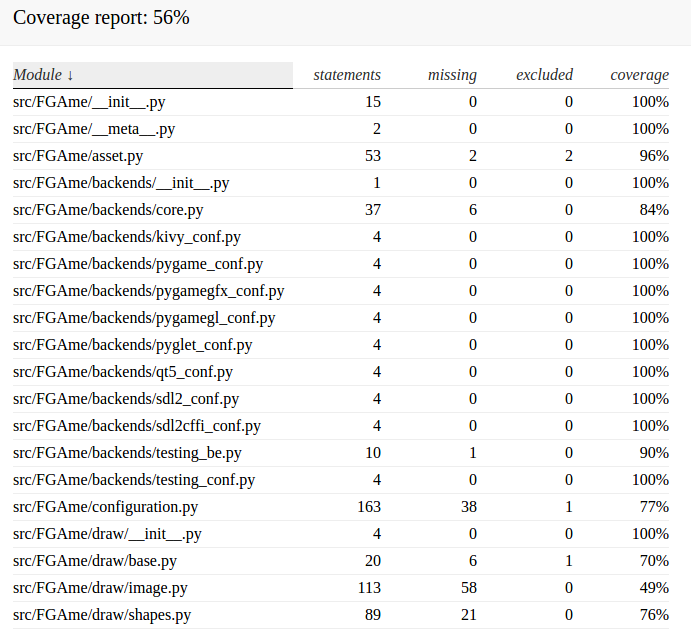
\includegraphics[scale=0.6]{figuras/coverage}
\caption{Cobertura do código}
\label{Rotulo}
\end{figure}


{\LARGE \textbf{Teste da classe Body}}

\begin{lstlisting}

from FGAme.tests.physics import test_particle as base
from FGAme.physics.bodies import Body
from smallshapes.tests import abstract as shape_tests
from FGAme.mathtools import vec
import pytest

class TestBody(base.TestParticle, shape_tests.TestSolid):
    base_cls = Body

    def test_aabb_limits_aliases(self, obj):
        assert obj.xmin == obj.left
        assert obj.xmax == obj.right
        assert obj.ymin == obj.bottom
        assert obj.ymax == obj.top

    def test_aabb_coords_setters(self, obj):
        pos = obj.pos
        obj.xmin += 10
        assert obj.x == obj.pos.x

    ## methods from physics/utils.py

    def test_center_mass(self):

        from FGAme.physics.utils import center_of_mass

        b1 = Body(pos=(0, 30), mass=1)
        b2 = Body(pos=(10, 0), mass=3)

        vector = vec(7.5,7.5)

        assert center_of_mass(b1, b2) == vector

    def test_mass(self):

        from FGAme.physics.utils import mass

        b1 = Body(pos=(0, 30), mass=1)
        b2 = Body(pos=(10, 0), mass=3)

        assert mass(b1,b2) == 4

    def test_inertia(self):

        from FGAme.physics.utils import inertia

        b1 = Body(mass=1, inertia=2)
        b2 = Body(pos=(1, 0), mass=3, inertia=1)

        assert inertia(b1, b2) == 3.75

    def test_momentumP(self):

        from FGAme.physics.utils import momentumP

        b1 = Body(pos=(2, 0), mass=1)
        b2 = Body(pos=(-1, 0), mass=2)

        vector = vec(0.0,0.0)

        assert momentumP(b1, b2) == vector

    def test_momentumL(self):

        from FGAme.physics.utils import momentumL

        b1 = Body(mass=1)
        b2 = Body(pos=(-1, 0), mass=2)

        with pytest.raises(Exception):
            momentumL(b1, b2)

    def test_energyK(self):

        from FGAme.physics.utils import energyK

        b1 = Body(pos=(2, 0), mass=1)
        b2 = Body(pos=(-1, 0), mass=2)

        assert energyK(b1,b2) == 0.0

    def test_linearK(self):

        from FGAme.physics.utils import linearK

        b1 = Body(pos=(2, 0), mass=1)
        b2 = Body(pos=(-1, 0), mass=2)

        assert linearK(b1,b2) == 0.0

    def test_angularK(self):

        from FGAme.physics.utils import angularK

        b1 = Body(pos=(2, 0), mass=1)
        b2 = Body(pos=(-1, 0), mass=2)

        assert angularK(b1,b2) == 0.0

    def test_energyU(self):

        from FGAme.physics.utils import energyU

        b1 = Body(pos=(2, 0), mass=1)
        b2 = Body(pos=(-1, 0), mass=2)

        assert energyU(b1,b2) == 0.0

    def test_energy(self):

        from FGAme.physics.utils import energy

        b1 = Body(pos=(2, 0), mass=1)
        b2 = Body(pos=(-1, 0), mass=2)

        assert energy(b1,b2) == 0.0

    def test_safe_div(self):

        from FGAme.physics.utils import safe_div

        assert safe_div(10,2) == 5
        assert safe_div(10,0) == float('inf')

    def test_normalize_flag_value(self):

        from FGAme.physics.utils import normalize_flag_value

        assert normalize_flag_value('has_external_alpha') != None
        assert normalize_flag_value(2) == 2

    def test_aslist(self):

        from FGAme.physics.utils import aslist

        assert aslist('hello') == 'hello'
        assert aslist(['hello', 'test']) ==  ['hello', 'test']

        with pytest.raises(Exception):
            aslist()
\end{lstlisting}



{\LARGE \textbf{Teste dos módulos de Texto}}

\begin{lstlisting}
from FGAme.utils.text import snake_case
from FGAme.utils.util import popattr

def test_snake_case():
    assert snake_case("TestSnakeCase") == "test_snake_case"

def test_popattr():

	from FGAme.physics.bodies import Body

	b1 = Body(pos=(0, 30), mass=1)

	result = popattr(b1,'position')

	assert result == None 
	## example of deletable attr on FGAme?

\end{lstlisting}


{\LARGE \textbf{Teste da classe Objects}}

\begin{lstlisting}
from FGAme.physics.simulation import Simulation
from FGAme.world.world import World

def test_simulation_enforce_max_speed():
    speed = 10.0
    w = World(max_speed = speed)
    p = w.add.poly(vertices=[(0,0), (1,1), (0,2)], vel=(200, 200), pos=(0,0))
    w._simulation.enforce_max_speed()
    assert p._vel.norm_sqr() > speed ** 2

def test_simulation_gravity():
    gravity = (0, -10.0)
    w = World(gravity=gravity)
    p = w.add.regular_poly(N=6, length=2.0, pos=(0,0), mass=1.0)
    w.update(0.1)
    assert p._acceleration == gravity

def test_simulation_discard_object():
    gravity = (0, -10.0)
    w = World(gravity=gravity)
    p = w.add.regular_poly(N=6, length=2.0, pos=(0,0), mass=1.0)
    w._simulation.discard(p)
    w.update(0.1)
    assert p._acceleration != gravity
\end{lstlisting}


{\LARGE \textbf{Teste da classe Simulation e World}}

\begin{lstlisting}
from FGAme.physics.
from FGAme.physics.simulation import Simulation
from FGAme.world.world import World

def test_simulation_enforce_max_speed():
    speed = 10.0
    w = World(max_speed = speed)
    p = w.add.poly(vertices=[(0,0), (1,1), (0,2)], vel=(200, 200), pos=(0,0))
    w._simulation.enforce_max_speed()
    assert p._vel.norm_sqr() > speed ** 2

def test_simulation_gravity():
    gravity = (0, -10.0)
    w = World(gravity=gravity)
    p = w.add.regular_poly(N=6, length=2.0, pos=(0,0), mass=1.0)
    w.update(0.1)
    assert p._acceleration == gravity

def test_simulation_discard_object():
    gravity = (0, -10.0)
    w = World(gravity=gravity)
    p = w.add.regular_poly(N=6, length=2.0, pos=(0,0), mass=1.0)
    w._simulation.discard(p)
    w.update(0.1)
    assert p._acceleration != gravity
\end{lstlisting}


{\LARGE \textbf{Teste da classes de Backend}}

\begin{lstlisting}
import pytest
from FGAme.backends import get_backend_classes
from FGAme.backends import testing_be
from FGAme import conf


def test_find_correct_backend_classes():
    D = get_backend_classes('testing')
    assert D == {
        'input': testing_be.EmptyInput,
        'mainloop': testing_be.MainLoop,
        'screen': testing_be.EmptyCanvas,
    }


@pytest.mark.pygame
def test_find_pygame_backend():
    from FGAme.backends import pygame_be

    D = get_backend_classes('pygame')
    assert D == {
        'input': pygame_be.PyGameInput,
        'mainloop': pygame_be.PyGameMainLoop,
        'screen': pygame_be.PyGameCanvas,
    }

def test_show_screen():
    conf.show_screen()
    assert conf._screen_object

def test_set_resolution():
    conf.set_resolution(800,600)
    screen = conf.get_screen()
    assert screen.width == 800
    assert screen.height == 600

def test_set_resolution_fullscreen():
    with pytest.raises(Exception):
        conf.set_resolution('fullscreen')

def test_set_resolution_already_defined():
    with pytest.raises(Exception):
        conf.set_resolution(400,400)

def test_set_framerate():
    value = 30
    conf.set_framerate(value)
    assert conf._physics_fps == value
    assert conf._physics_dt == 1/value

def test_get_framerate():
    assert conf._physics_fps == 30

def test_set_frame_duration():
    value = 1
    conf.set_frame_duration(value)
    assert conf._physics_fps == value
    assert conf._physics_dt == 1/value

def test_get_frame_duration():
    assert conf._physics_dt == 1

def test_get_backend():
    backend = conf.get_backend()
    assert backend == 'testing'
\end{lstlisting}



{\LARGE \textbf{Teste da classe Simulation e World}}

\begin{lstlisting}

import pytest
from FGAme.world.tracker import Tracker
from FGAme.world.world import World

def test_tracker_energy_tracker_not_none():
    w = World()
    t = Tracker(w)
    assert t.energy()

def test_energy_tracker_method():
    w = World()
    w._simulation._kinetic0 = 1.0
    w._simulation._potential0 = 1.0
    w._simulation._interaction0 = 1.0
    t = Tracker(w)
    e1 = t.energy()
    e2 = w.track.energy()
    assert e1() == e2()

def test_energy_tracker_raises_division_by_zero():
    w = World()
    w._simulation._kinetic0 = 0
    w._simulation._potential0 = 0
    w._simulation._interaction0 = 0
    e1 = w.track.energy()
    with pytest.raises(ZeroDivisionError):
        e1()

def test_energy_tracker_default_kinetic_energy():
    w = World()
    w._simulation._kinetic0 = None
    w._simulation._potential0 = 0
    w._simulation._interaction0 = 0
    e1 = w.track.energy()
    assert e1() == None
\end{lstlisting}

\end{anexosenv}



% Definindo novas cores
\definecolor{verde}{rgb}{0,0.5,0}
% Configurando layout para mostrar codigos C++
\lstset{
  language=ruby,
  basicstyle=\ttfamily\small,
  keywordstyle=\color{blue},
  stringstyle=\color{verde},
  commentstyle=\color{red},
  extendedchars=true,
  showspaces=false,
  showstringspaces=false,
  numbers=left,
  numberstyle=\tiny,
  breaklines=true,
  backgroundcolor=\color{green!10},
  breakautoindent=true,
  captionpos=b,
  xleftmargin=0pt,
}
\pagestyle{empty}

\begin{anexosenv}

\chapter{Configuração da integração continua}
\label{sec:anexo2}

\begin{figure}[!htb]
\begin{lstlisting}
{
  "language": "python",
  "python": "nightly",
  "sudo": "required",
  "env": "AUDIODEV=null",
  "install": [
    "sudo apt-get install python3-dev mercurial",
    "sudo apt-get update",
    "sudo apt-get -y install mercurial",
    "hg clone https://bitbucket.org/pygame/pygame",
    "sudo apt-get update",
    "sudo apt-get install -y python3-dev python3-numpy libsdl-image1.2-dev libsdl-mixer1.2-dev libsdl-ttf2.0-dev libsmpeg-dev libsdl1.2-dev libportmidi-dev libswscale-dev libavformat-dev libavcodec-dev libfreetype6-dev",
    "pip3 install hg+http://bitbucket.org/pygame/pygame",
    "pip install pgzero",
    "pip install pip -U",
    "pip install .[dev] -r requirements.txt",
    "pip install coveralls pytest-cov",
    "pip install Pillow",
    "pip install FGAme"
  ],
  "script": [
    "py.test src/FGAme/tests/ --cov"
  ],
  "after_success": [
    "coveralls"
  ],
  "group": "stable",
  "dist": "precise",
  "os": "linux"
}
\end{lstlisting}
\end{figure}

\begin{figure}[!htb]
\centering
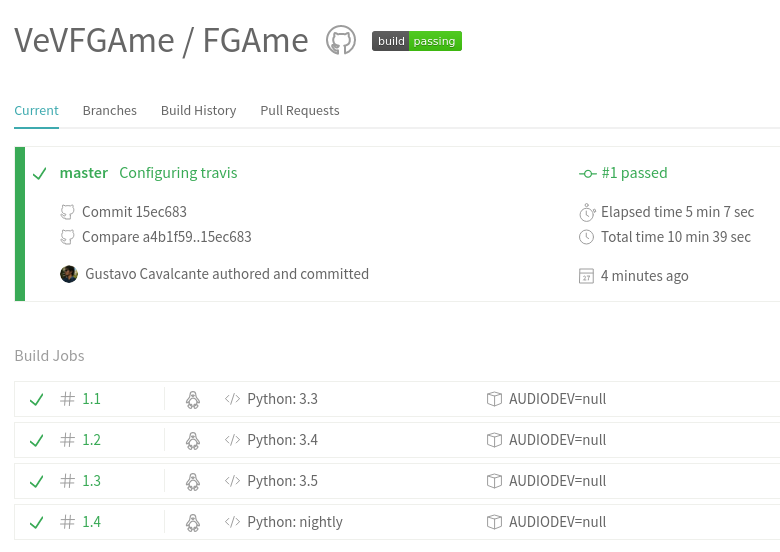
\includegraphics[scale=0.6]{figuras/build}
\caption{\textit{Build} do Travis passando corretamente.}
\label{Rotulo}
\end{figure}

\end{anexosenv}